\chapter{Segurança em Redes de Computadores} \label{ch:segurança}
\section{Definições} \label{sec:definições}

Para entendemos melhor o que é segurança da informação, precisamos conceituar alguns termos que serão detalhados abaixo \cite{esr-gestao}:

\begin{alineas}
 \item \textbf{Incidente de segurança}: qualquer evento oposto a segurança; por exemplo, ataques de negação de serviços (Denial of Service - DoS), roubo de informações, vazamento e obtenção de acesso não autorizado a informações;
 \item \textbf{Ativo}: qualquer coisa que tenha valor para a organização e para seus negócios. Alguns exemplo: banco de dados, softwares, equipamentos (computadores e notebooks), servidores, elementos de redes (roteadores, switches, entre outros), pessoas, processos e serviços;
 \item \textbf{Ameaça}: qualquer evento que explore vulnerabilidades. Causa potencial de um incidente indesejado, que pode resultar em dano para um sistema ou organização;
 \item \textbf{Vulnerabilidade}: qualquer fraqueza que possa ser explorada e comprometer a segurança de sistemas ou informações. Fragilidade de um ativo ou grupo de ativos que pode ser explorada por uma ou mais ameaças. Vulnerabilidades são falhas que permitem o surgimento de deficiências na segurança geral do computador ou da rede. Configurações incorretas no computador ou na segurança também permitem a criação de vulnerabilidades. A partir dessa falha, as ameaças exploram as vulnerabilidades, que, quando concretizadas, resultam em danos para o computador, para a organização ou para os dados pessoais;
 \item \textbf{Risco}: probabilidade de uma ameaça se concretizar;
 \item \textbf{Ataque}: qualquer ação que comprometa a segurança de uma organização;
 \item \textbf{Impacto}: consequência de um evento.
\end{alineas}

Segurança da Informação proteção das informações, sistemas, recursos e demais ativos contra desastres, erros (intencionais ou não) e manipulação não autorizada, objetivando a redução da probabilidade e do impacto de incidentes de segurança.

Segundo a norma ISO/IEC 27002 \cite{isoiec27002}, segurança da informação é a preservação da confidencialidade, da integridade e da disponibilidade da informação; adicionalmente, outras propriedades, tais como autenticidade, responsabilidade, não repúdio e confiabilidade, podem também estar envolvidas.

Dentre vários conhecimentos que um profissional de segurança deve possuir, o conceito mais básico e considerado o pilar de toda a área de segurança corresponde à sigla CID (Confidencialidade, Integridade e Disponibilidade), de modo que um incidente de segurança é caracterizado quando uma dessas áreas é afetada \cite{seg-redes-sistemas}. Abaixo será detalhado cada item.

\begin{alineas}
 \item \textbf{Confidencialidade}: termo ligado à privacidade de um ativo ou recurso, que deve ser acessível somente por pessoas ou grupos autorizados;
 \item \textbf{Integridade}: possui duas definições, a primeira está relacionada com o fato da informação ter valor correto, a segunda, está ligada à inviolabilidade da informação;
 \item \textbf{Disponibilidade}: está relacionada ao acesso à informação, que deve está disponível quando necessária.
\end{alineas}

Dois dos termos citados são fáceis de ser monitorados pois é perceptível para o usuário: a integridade (identificar se uma informação foi alterada) e a disponibilidade (tentando acessar um serviço e verificando se o mesmo está respondendo adequadamente). No entanto, só é possível identificar se houve quebra da confiabilidade através de auditorias, analisando os registros de acesso (se houver), tornando a identificação complicada e em muitos casos impossível \cite{seg-redes-sistemas}.

Além dos conceito listados, a literatura moderna considera mais alguns conceitos auxiliares, temos:

\begin{alineas}
 \item \textbf{Autenticidade}: garantia que uma informação, produto ou documento foi elaborado ou distribuído pelo autor a quem se atribui;
 \item \textbf{Legalidade}: garantia de que ações sejam realizadas em conformidade com os preceitos legais vigentes e que seus produtos tenham validade jurídica;
 \item \textbf{Não repúdio}: conceito bastante utilizado em certificação digital, onde o emissor de uma mensagem não pode negar que a enviou;
 \item \textbf{Privacidade}: habilidade de uma pessoa controlar a exposição e a disponibilidade de informações acerca de si.
\end{alineas}

\section{Cenário Geral} \label{sec:cenario-geral}
%apresentar o cenário geral de uma rede conectada a Internet
\section{Pontos de Vulnerabilidade} \label{sec:pontos-vulnerabilidade}
%Ex.: Roteador, firewall, clientes e suas aplicações,
\section{Ataques Comuns à Redes de Computadores} \label{sec:ataques-comuns}

Nessa seção será descritos os ataques mais comuns à redes e serviços de organizações privadas e públicas, financeiras ou acadêmicas. Para licitar os ataques dessa seção, levou-se em consideração as estatísticas divulgada pelo CERT.br (\autoref{fig:cert}).

O CERT.br é o grupo de resposta a incidentes de segurança para a internet brasileira, mantido Comitê Gestor da Internet no Brasil. Atua na notificação e tratamento de incidentes de segurança dando apoio no processo de resposta. Além disso, faz um trabalho de conscientização e treinamento sobre problemas de segurança no Brasil. 

\begin{figure}[htb]
 \centering
 \caption{Estatísticas de ataques reportadas ao CERT.br}
 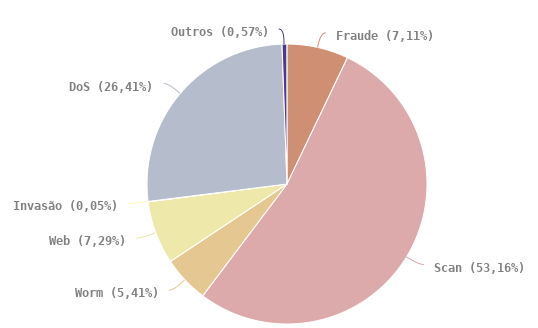
\includegraphics[scale=.5]{incidentes-reportados.png}
 \legend{Fonte: \cite{tipos-ataques:certs.br}}
 \label{fig:cert}
\end{figure}

O CAIS é responsável por zela pela segurança da rede Ipê (infraestrutura de rede dedicada à comunidade brasileira de ensino superior), detectando, resolvendo e prevenindo incidentes de segurança. Além disso, tem o papel de orientar (através de publicações de cartilhas) e disseminar boas práticas de segurança da informação, educando e conscientizando usuários de todos os níveis sobre os principais riscos em segurança da informação \cite{cais}.

\subsection{\textit{Scanners}} \label{sec:varredura}

Conforme tratado na \autoref{sec:definições}, uma vulnerabilidade é a fraqueza em sistemas de informação, procedimentos de segurança do sistema e controles internos, ou aplicação que pode ser explorada tendo como origem uma ameaça. 

\textit{Scanners} são programas usados para varrer uma rede à procura de computadores (tanto pessoais como servidores) com alguma vulnerabilidade. Podemos dividir os \textit{scanners} em dois tipos \cite{univhacker}: 

\begin{alineas}
\item \textbf{\textit{scanner} de portas TCP/IP abertas (ou \textit{portscanner})}: cada serviço de rede que estiver disponível em uma determinada máquina é uma porta de entrada em potencial. Existem um total de 128 mil porta, sendo 65536 portas para o protocolo TCP e 65536 portas para o protocolo UDP. O \textit{portscanner} verifica quais portas TCP/IP estão abertas com o objetivo de determinar quais serviços de rede TCP/IP disponíveis. Quase todas as técnicas de \textit{portscanning} valem-se de sinais (ou \textit{flags}), TCP, UDP ou ICMP, e a partir da análise desses sinais, os \textit{scanners} retiram informações sobre o sistema; \cite{univhacker}
\item \textbf{\textit{scanner} de vulnerabilidades conhecidas}: Um vez determinados os serviços que uma máquina disponibiliza na rede entra em cena o \textit{scanner} de vulnerabilidade. A ideia é checar, através de uma lista de falhas conhecidas, se o sistema está ou não executando um serviço com problemas \cite{univhacker}. 
\end{alineas}

Normalmente, essas ferramentas funcionam em três estágios \cite{}:

\begin{alineas}
 \item \textbf{Configuração}: aqui será definido o endereço IP do alvo ou a URL (Uniform Resource Locator) da aplicação Web e demais parâmetros, como, por exemplo, utilização de \textit{proxy}.
 \item \textbf{Rastreamento}: esse estágio é especifico de \textit{scanners} de vulnerabilidade de aplicações web, nele, o \textit{scanner} chama a primeira página web e então examina seu código procurando \textit{links}. Cada \textit{link} encontrado é registrado e este procedimento é repetido várias vezes até que \textit{links} e páginas não sejam mais encontrados.
 \item \textbf{Exploração}: vários testes são executados e as requisições e respostas são armazenadas e analisadas. Ao final, os resultados são exibidos ao usuário e podem ser salvos para uma análise posterior. 
\end{alineas}


Um bom \textit{scanner} de vulnerabilidade verifica itens como \cite{univhacker}: 

\begin{alineas}
\item \textbf{Erros comuns de configuração}: portas não utilizadas por nenhum serviço abertas;
\item \textbf{Configurações e senhas-padrões}: instalação de softwares deixando-os com as configurações de fabrica (com usuário e senha-padrão), por exemplo, usuário: admin, senha: admin. Outro problema é deixar serviços desnecessários ativados;
\item \textbf{Combinação óbvias de usuário e senha}: Usuário comuns tendem a colocar senhas fáceis de lembrar;
\item \textbf{Vulnerabilidades divulgadas}: Sempre que uma falha de segurança é divulgada há uma corrida dos desenvolvedores para saná-las. Em paralelo, existem \textit{hackers} que querem chegar aos sistemas vulneráveis antes de serem consertados.
\end{alineas}

\subsection{\texit{Exploit}} \label{sec:exploração}

\begin{alineas}
 \item \textbf{Configuração}: aqui será definido o endereço IP do alvo ou a URL (Uniform Resource Locator) da aplicação Web e demais parâmetros, como, por exemplo, utilização de \textit{proxy}.
 \item \textbf{Rastreamento}: esse estágio é especifico de \textit{scanners} de vulnerabilidade de aplicações web, nele, o \textit{scanner} chama a primeira página web e então examina seu código procurando \textit{links}. Cada \textit{link} encontrado é registrado e este procedimento é repetido várias vezes até que \textit{links} e páginas não sejam mais encontrados.
 \item \textbf{Exploração}: vários testes são executados e as requisições e respostas são armazenadas e analisadas. Ao final, os resultados são exibidos ao usuário e podem ser salvos para uma análise posterior. 
\end{alineas}

Os \textit{Scanners} de vulnerabilidades automatizados contêm, e atualizam regularmente, enormes bancos de dados de assinaturas de vulnerabilidades conhecidas para basicamente tudo o que está recebendo de informações em uma porta de rede, inclusive sistemas operacionais, serviços e aplicativos web. Eles podem até detectar vulnerabilidades no software do lado do cliente mediante credenciais suficientes, uma estratégia que pode ser útil em estágios posteriores do ataque, quando o invasor pode estar interessado em expandir ainda mais sua base de operações, comprometendo contas adicionais de usuário privilegiado \cite{hackers:stuart-joel}.

Diante da lista de vulnerabilidades encontradas com os \textit{scanners}, próximo passo seria usar um \textit{exploit} adequado. Os \textit{exploit} são pequenos utilitários usados para explorar vulnerabilidades específicas, podendo serem usados de forma \textit{"stand alone"}, ou seja, serem usados diretamente, ou podem ser incorporados à \textit{malwares} \cite{exploit:cassio}.

\subsection{Força Bruta} \label{sec:forçabruta}

Na segurança da informação, a autenticação é umas das áreas-chaves onde há a distinção de usuários autorizados de outros não-autorizados, tendo como principal vantagem ser de fácil implementação, não requerendo equipamentos, como leitores biométricos \cite{denise-lilian}.

Na literatura sobre segurança da informação, o fator humano é considerado o elo mais fraco. Muitos usuários, por conveniência, criam senhas de acesso fáceis e, em muitos casos, única para acessar diversos sistemas. Nesse ponto que \textit{hackers} iram atuar para ter acesso não-autorizado ao sistema. 

Existem três métodos mais usados por programas de quebra de senha: ataques de dicionário (ou lista de palavras), ataques híbridos e ataques de força-bruta. Nos ataques por dicionários, utilizam-se listas de palavras comuns: nomes próprios, marcas conhecidas, gírias, nomes de canções, entre outros, tais elementos conseguidos por engenharia social \cite{univhacker}. 

 Um ataque de força bruta consiste em gerar todas as permutações e combinações possíveis de senha, criptografar cada uma e comparar a senha gerada com a senha criptografada original até encontrar uma que seja igual \cite{md5crack2012}. 

 Esse tipo de ataque é facilmente detectável pois, além de gerar uma alta carga no servidor, gera uma grande quantidade de registros de logs. No entanto, caso a pessoa má intencionada, de alguma outra forma, tenha acesso ao arquivo de \textit{hash} ou a tabela de usuário de um banco de dados, com as senha criptografadas do sistema, ela pode usar o ataque de força bruta no arquivo em qualquer máquina, assim, impossibilitando a detecção do ataque.

 Muitos sistemas já possuem formas de contornar esse tipo de ataque, por exemplo, bloqueio de usuário ao errar a palavra-chave por uma certa quantidade de vezes. Outra forma, é colocar um tempo de expiração da senha, por exemplo, a senha deve ser trocada a cada trinta dias por uma diferente e nunca usada anteriormente, dessa maneira, inviabilizando a quebra de senha por força bruta. 

 \subsection{Desfiguração de páginas} \label{sec:desfiguração}

 A desfiguração de páginas, \textit{defacement} ou pichação ocorre quando o conteúdo da página \textit{web} de um site é alterado. O atacante (\textit{defacer}) consegue fazer alterações em páginas explorando vulnerabilidade nas aplicações \textit{web} que permite injeção de \textit{script} malicioso ou através de furto de senha de acesso à interface \textit{web} usadas para administração remota \cite{certs-ataques}.

 Nos serviços \textit{web}, como por exemplo, apache2 existe um usuário especial, comumente chamado de www-data ou algo semelhante. O servidor \textit{web}, na maioria das vezes, precisa apenas de permissões de leitura nos arquivos porém muitos gerentes de sistemas cujo a conscientização sobre segurança é insuficiente, designa permissões errôneas (escrita ou alteração), e caso haja um comprometimento, através, por exemplo, de injeção de código remoto PHP, do servidor, o atacante poderá alterar a maioria dos arquivos. A ocorrência amplamente disseminada de ataques de desfiguração de páginas Web é uma consequência direta dessa prática \cite{seguranca:william-lawrie}.

 Em 2010, o site Zone-h registrou mais de 1,4 milhões de páginas desfiguradas, muitas delas associadas a ataques \textit{Cross-site scripting} (XSS). Os \textit{defacements} são considerados ataques passivos pois é gerado apenas uma mensagem na tela \cite{angelo-xss}.

 \subsection{Negação de Serviços} \label{sec:negação}
 
Um ataque de negação de serviço (\textit{Denial of Service} - DoS) tem como principal objetivo deixar um serviço (servidor web, banco de dados) ou recurso (memória, processador)  indisponível, impossibilitando que usuário legítimos tenham acesso a esses recursos. Para tal, o atacante gera diversas requisições inúteis para o servidor, consumindo seus recursos até que o serviço não esteja mais disponível ou degradando a qualidade do serviço \cite{cryptsec}.

Esse tipo de ataque pode gerar grandes prejuízos financeiros para as empresas, principalmente \textit{e-commence}, pois enquanto o sistema está fora ou com uma resposta lenta, as transações financeiras são prejudicadas. Com isso, cria-se também, uma insatisfação pelo usuário do serviço prestado pela empresa.

Existe um forma mais sofisticada de ataque de Negação de Serviço chamada Negação de Serviço Distribuído (\textit{Distributed Denial of Services} - DDoS), enquanto o DoS básico as requisições partem de apenas uma fonte (Figura \ref{dos}), no DDoS o atacante tem acesso a um grande número de computadores (\textit{zombies}) explorando suas vulnerabilidades criando o que chamamos de \textit{botnet} (Figura \ref{ddos}). Com isso, basta o atacante indicar as coordenadas de um ou mais alvos para o ataque \cite{zargarjoshitipper}. 

 \subsection{Malwares} \label{sec:malwares}

 Os \textit{malwares}, também conhecidos como \textit{softwares} maliciosos, são um grande problema para sistemas de informação, sua existência ou execução tem consequências negativas ou involuntárias. Os \textit{malwares} mais conhecidos são os vírus, worms e trojans.

 É importante entender o funcionamento e o comportamento desses códigos maliciosos para, a partir daí, buscar soluções contra esse ataque. Existe dois tipos de análise: análise estática, requer uma verifica linha a linha do código malicioso, geralmente o código não está disponível e até mesmo se estiver, o autor do \textit{malware} muitas vezes ofusca o código, tornando esse tipo de análise difícil. Por outro lado, existe a análise dinâmica, o analista monitora a execução e o comportamento do \textit{malware}, esse tipo de análise é imune a ofuscação de código \cite{encycrypt}.

 O Vírus é um programa que se propaga inserindo cópias de si mesmo e se tornando parte de outros programas e arquivos. Para dar continuidade ao processo de infecção, o vírus depende da execução do programa ou arquivo hospedeiro. O principal meio de propagação desse tipo de \textit{software} malicioso são as mídias removíveis, como, por exemplo, pen-drives \cite{certs-malwares}.

O Worm é um \textit{malware} que se propaga através de e-mails, sites ou \textit{software} baseados em rede, explorando as vulnerabilidades das aplicações. Uma das principais características desse tipo de \textit{software} é a propagação automática, ou seja, sem a intervenção do usuário \cite{detectingworm}. 

O Trojan ou Cavalo de Troia são programas que precisam ser explicitamente executados para serem instalados no computador. Esse \textit{malware} se disfarça de um programa benigno, por exemplo, cartões virtuais animados, álbuns de fotos, jogos e protetores de tela que ao serem executados o trojan é instalado sem o consentimento do usuário. No entanto, o atacante, após invadir um computador, pode instalar o trojan  alterando as funções já existentes de programas para executarem ações maliciosas \cite{certs-malwares}.

 \section{Ferramentas para Avaliação de Segurança} \label{sec:ferramentas}
 %Nmap, Metasploit, Pytbull

 Nessa seção será descrito as ferramentas auxiliares utilizadas para geração de ataques \autoref{sec:ataques} com objetivo de testar e validar as configurações das ferramentas de IDPS estudas. 

 \subsection{Nmap} \label{sec:nmap}

 O Nmap é uma ferramente de código aberto utilizada para auditoria de segurança e descoberta de rede. A ferramenta é capaz de determinar quais \textit{hosts} estão disponíveis na rede, quais serviços cada \textit{host} está oferecendo, incluindo nome e versão da aplicação, o sistema operacional usado, dentre outras características.  

 Muitos administradores de sistemas utilizam o Nmap para tarefas rotineiras como, criação de inventário de rede, gerenciamento de serviços, visto que é de suma importância manter os mesmos atualizados e monitoramento de \textit{host}.

 Diversos parâmetros podem ser utilizados com o Nmap, possibilitando realizar varreduras das mais variadas maneiras, dependendo do tipo desejado. A lista completa de opções podem ser consultadas na documentação oficial que vem junto da ferramenta ou no site do projeto \cite{nmap}. 

 Na execução do Nmap, o que não for opção ou argumento da opção é considerado especificação do \textit{host} alvo. O alvo pode ser um ou vários, usando uma notação de intervalo por hífen ou uma lista separada por vírgula. Os \textit{hosts} alvos também podem ser definidos em arquivos.

 O resultado do Nmap é uma tabela de portas e seus estados (\autoref{fig:nmap-exemplo}). As portas podem assumir quatro estados, temos: aberto (\textif{open}), significa que existe alguma aplicação escutando conexões; filtrado (\textit{filtered}), há um obstáculo na rede, podendo ser algum \textit{firewall}, que impossibilita que o Nmap determine se a porta está aberta ou fechada; fechado (\textit{closed}), não possui aplicação escutando na porta; não-filtrado (\textit{unfilterd}), a porta responde requisição porém o Nmap não consegue determinar se estão fechadas ou abertas \cite{nmap}

 \begin{figure}[htb]
  \centering
  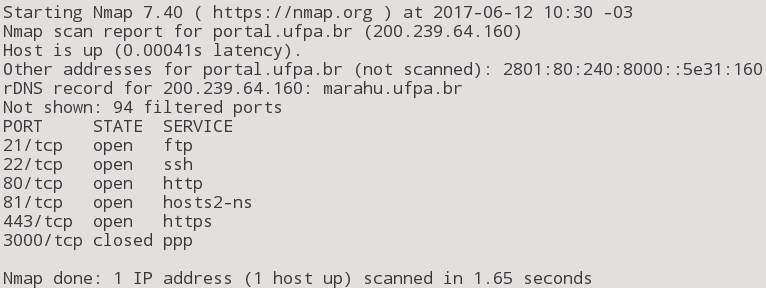
\includegraphics[scale=.5]{nmap.png}
  \caption{Exemplo de saída do Nmap}
  \label{fig:nmap-exemplo}
 \end{figure}

 \subsection{Metasploit Framework} \label{sec:metasploit}

 O Metasploit é um \textit{framework} de código aberto cujo principio básico é desenvolver e executar \textit{exploit} contra alvos remotos e fornecer uma lista de vulnerabilidades existentes no alvo. É uma ferramenta que combina diversos \textit{exploits} e payloads dentro de um local, ideal para levantamento de segurança de serviços e testes de penetração \cite{metasploit:yash}.  

 O Metasploit possui uma biblioteca divida em três partes: \textbf{Rex}: É a biblioteca fundamental, a maioria das tarefas executadas pelo \textit{framework} usaram essa biblioteca; \textbf{MSF Core}: É o \textit{framework} em si, possui, por exemplo, gerenciador de módulos e a base de dados; \textbf{MSF Base}: Guarda os módulos, sejam eles, \textit{exploit}, \textit{encoders} (ferramentas usadas para desenvolver o \textit{payloads}) e os \textit{payloads}. Além disso, são guardadas informações de configuração e sessões criadas pelos \textit{exploits}. A arquitetura é mostrada com mais detalhes na \autoref{fig:metasploit-arquitetura}. 

 Os módulos são divididos da seguinte maneira: Payload: são código executados no alvo remotamente; Exploit: explora \textit{bugs} ou vulnerabilidade existente em aplicações do alvo; Módulos Auxiliares: usado para escanear as vulnerabilidades e executar várias tarefas; Encoder: codifica o \textit{payload} para evitar qualquer tipo de detecção pelo anti vírus.

 \textbf{Interface}: Disponibiliza a parte gráfica para o usuário;

 \begin{figure}[!htb]
  \centering
  \caption{Arquitetura do Metasploit}
  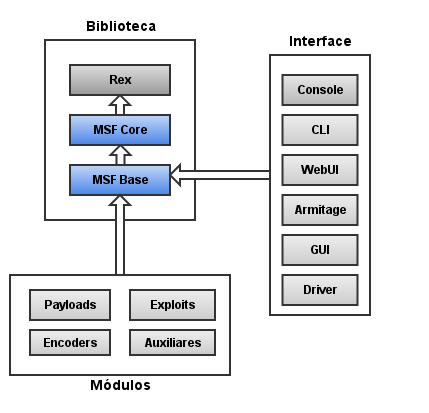
\includegraphics[scale=.6]{metasploit_arquitetura.png}
  \legend{}
  \label{fig:metasploit-arquitetura}
 \end{figure}

 \subsection{Pytbull} \label{sec:pytbull}

 O Pytbull é um \textit{framework} para teste de IDPS, capaz de determinar a capacidade de detecção e bloqueio do mesmo, além de fazer uma comparação entre diversas soluções e verifica as configurações \cite{pytbull}. O \textit{framework} Pytbull possui cerca de 300 testes agrupados em 11 módulos, temos:

 \begin{alineas}
  \item \textbf{badTraffic}: pacotes não compatíveis com a RFC são enviados para o servidor para testar como os pacotes são processados; 
  \item \textbf{bruteForce}: testa a capacidade do IDPS de rastrear ataques de força bruta;
  \item \textbf{clientSideAttacks}: usa um \textit{shell} reverso para fornecer ao servidor instruções para baixar arquivos maliciosos; 
  \item \textbf{denialOfService}: testa a capacidade do IDPS de proteger contra tentativas de DoS; 
  \item \textbf{evasionTechniques}: testa a capacidade do IDPS de detectar técnicas de evasão; 
  \item \textbf{fragmentedPackets}: várias cargas úteis fragmentadas são enviadas ao servidor para testar sua capacidade de recomposição e detectar os ataques; 
  \item \textbf{ipReputation}: testa a capacidade do servidor detectar tráfego de servidores com reputação baixa;
  \item \textbf{normalUsage}: cargas úteis que correspondem a uso normal; 
  \item \textbf{pcapReplay}: permite reproduzir arquivos pcap; 
  \item \textbf{shellCodes}: envia \textit{shellcodes} para o servidor na porta 21/ftp testando a capacidade de detectar e/ou bloquear o mesmo; 
  \item \textbf{testRules}, testa a base de assinaturas configuradas no servidor IDPS.
 \end{alineas}

 Existem basicamente 5 tipos de testes: socket, abre um \textit{socket} em uma porta e envia o \textit{payload} para o alvo remoto na porta especificada; command, envia um comando para alvo remoto com a função python subprocess.call(); scapy, envia cargas úteis especificas baseadas na sintaxe de Scapy; client side attacks, usa um \textit{shell} reverso no alvo remoto e envia comandos para serem processados no servidor; pcap replay, permite reproduzir tráfego com base em arquivos de pcap.

 \begin{figure}[htb]
  \centering
  \caption{Arquitetura do \textit{framework} Pytbull}
  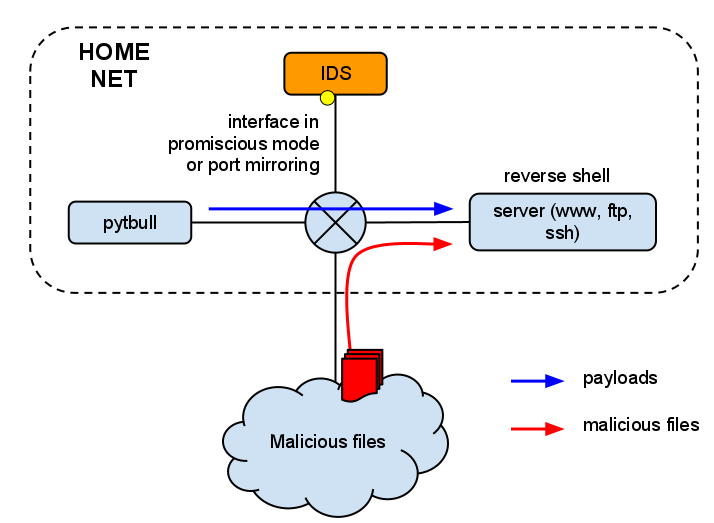
\includegraphics[scale=.4]{arquitetura_pytbull.png}
  \legend{}
  \label{fig:pytbull}
 \end{figure}

 \section{Conclusão}
 %Este capítulo apresentou
